\subsection{UIについて}
\label{tag:ui}
UIの基本的な部分は、魚本、大須賀、中村(2018)らの制作したネットワーク自己学習機能を採用した。これの概要を図\ref{fig:simu}に示す。

\begin{figure}[htbp]
  \begin{center}
    \resizebox{\textwidth}{!}{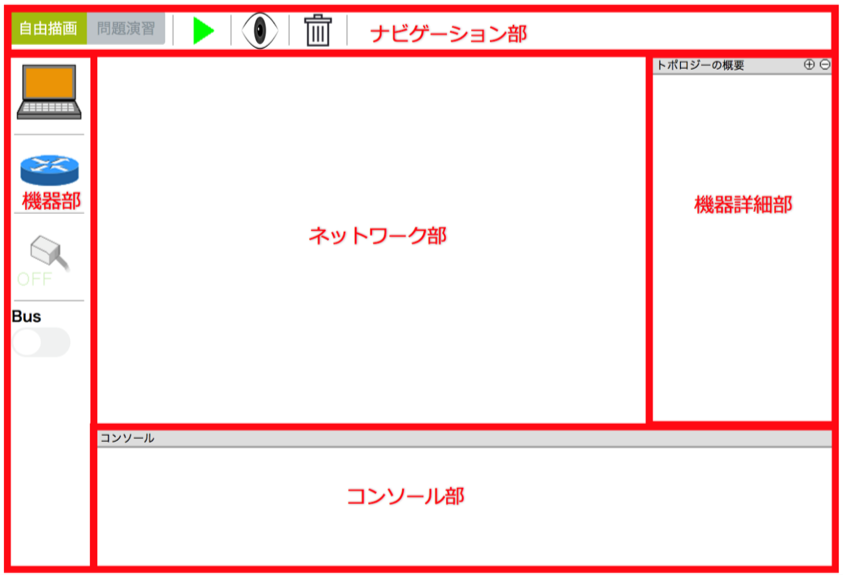
\includegraphics{img/simu.png}}
    \caption{ネットワーク自己学習機能 UI(差し替えます)}
    \label{fig:simu}
  \end{center}
\end{figure}

図\ref{fig:simu}のネットワーク自己学習機能は、実際にネットワークに関する学習を終えた学生に対しアンケートを行い、9割以上の学生がデザインについて見やすいと答えていた。これにより図\ref{fig:simu}のネットワーク自己学習機能のUIは変更する必要性がないと判断した。\\
 図\ref{fig:simu}は5つの部分に分けられており、機器部、ナビゲーション部、ネットワーク部、機器詳細部、コンソール部となっている。また、図\ref{fig:simu}では自由描画モードと問題演習モードの2つのモードが用意されている。自由描画モードの際、ナビゲーション部ではそれぞれのアイコンをクリックすることでモードの変更、構築したネットワークの正誤の判定、それぞれの機器の詳細情報の確認、すべての要素の削除を行うことができる。\\
 問題演習モードの際は、これに加え練習問題一覧の表示、現在の状況のセーブ、セーブした状態のロード、問題演習モードの終了を行うことができる。\\
 機器部では自由描画モードの際に、PCやルータのネットワーク部へのドロップ、LANモードのON,OFFの切り替えを行うことができる。LANモードがONの場合ネットワーク部へドロップした機器をLANでつなぐことができる。LANモードがOFFの場合、ネットワーク部では機器部からドロップした機器を自由に移動することができる。\\
ネットワーク部では構築されているネットワークのそれぞれの機器に必要な情報を追加する事ができる。これによって正しいネットワークを構築していくことが本ネットワーク自己学習機能の目的である。\\
 機器詳細部はネットワーク部に追加されたそれぞれの機器の情報を確認する部分である。トポロジーの詳細部分の横のプラスボタンを押すことで機器の詳細な情報の表示、マイナスボタンでその非表示を設定することができる。\\
 コンソール部は不可能な操作やエラーなどの不具合が起こった場合などにそれぞれの理由や結果などをコンソールとして入力される部分である。また、ナビゲーション部ののボタンを用いて、ネットワークの正誤を判定する際に、ネットワーク部に構築されたネットワークが正しいかかどうか、間違っている場合構築したネットワークのどこの部分が間違っているかを表示する。\\
 これらの機能により、学習者はPCを複数用意し、実際にネットワークを構築することなくネットワーク自己学習機能上で擬似的にネットワークの構築を行うことができる。これにより、知識として学習しただけでは分かりづらいネットワークの分野を、視覚的に構築することで実際のネットワークの構成などを理解する助けとなる。
